\documentclass[11pt,a4paper]{article}
\usepackage{fontspec}
\setmainfont{Noto Serif}
\setsansfont{Noto Sans}
\setmonofont{DejaVu Sans Mono}
\usepackage{graphicx}
\usepackage{amsmath}
\usepackage{booktabs}
\usepackage{needspace}
\usepackage{float}
\usepackage{array}
\usepackage{url}
% microtype disabled for stable text display
\usepackage{xcolor}
\usepackage[final]{acl}
\title{AquaGent: An Explainable AI Decision-Support Prototype for Atmospheric Water Harvesting}
\author{Zainab Alameri \quad\textbullet\quad Abubaker Baobaid\\Effat University\\CS3081 Artificial Intelligence}
\date{}
\begin{document}
\raggedbottom
\twocolumn[{
\begin{center}
{\LARGE\bfseries AquaGent: An Explainable AI Decision-Support Prototype\\for Atmospheric Water Harvesting\par}
\vspace{0.22cm}
{\normalsize Zainab Alameri \quad $\bullet$ \quad Abubaker Baobaid\\Effat University\\CS3081 Artificial Intelligence\par}
\vspace{0.45cm}
{\large\bfseries Abstract\par}
\vspace{0.12cm}
\end{center}
\begin{minipage}{0.94\textwidth}
\noindent\fontsize{10.3}{13.4}\selectfont
AquaGent is a software prototype that helps an operator choose between fog collection using Raschel-type mesh and water-vapor collection using a MOF-303 sorbent bed. The operator enters weather data, fog sensor readings, energy limits, operating time, and safety status through a Streamlit page. A Bayesian model estimates the chance of fog, including when sensor evidence is missing. Constraint Satisfaction Problem (CSP) rules reject plans that do not meet operating limits. The system compares the remaining plans using estimated water output and electricity use, then lets the operator approve or reject a recommendation. We ran 45 automated tests, all of which passed, and ten simulated scenarios. Six scenarios produced recommendations, two produced no feasible plan, and two returned input warnings. We also checked how changing selected inputs affects the estimated results. AquaGent demonstrates a clear decision process; its water and energy values are simulated estimates, not measured results from a working water-harvesting device.
\end{minipage}
\vspace{0.55cm}
}]
\section{Introduction and Motivation}
Access to clean water is a challenge in many dry regions. Besides rivers and groundwater, air may provide a small additional water source. However, collecting water from air is not one single process. A fog collector catches droplets that are already floating in the air. A sorbent device takes up water vapor and must later release and condense it. Each option needs different weather and equipment conditions.

For example, fog collection depends on fog events, wind, and the mesh area. A MOF-based device can work without visible fog, but its output also depends on the material, the heating or regeneration process, and how water is condensed. Published studies from Saudi Arabia and other locations show useful results for particular systems, but those results cannot simply be treated as predictions for Jeddah \citep{alzahrani2025,song2023}. Humidity alone cannot decide which method fits a site.

\newpage\noindent Our project asks a practical question: \emph{How can a software agent suggest a fog collector, a MOF sorbent bed, or no safe plan when weather information and available resources change?} To explore this, we built AquaGent, a Streamlit prototype. It uses a Bayesian sensor model to handle uncertain fog readings and a constraint satisfaction problem (CSP) to reject plans that do not meet operating limits. It then compares the remaining plans and shows the result to a human operator. This is a study of the decision process, not a physical water-harvesting experiment. The water and energy numbers are estimates based on stated assumptions.

We also compared four collection methods before focusing on fog and sorption. Their roles in our software are different: the Bayesian model deals with uncertain sensor readings, while CSP checks whether each plan is allowed. A plan can have a high chance of fog and still be rejected because of an energy or safety limit. The interface explains why plans are rejected.




\section{Related Work}
We reviewed work on fog collection and water-vapor harvesting before designing AquaGent. In a study of fog harvesting in Al-Baha, Saudi Arabia, \citet{alzahrani2025} looked at local conditions and possible collection sites. Their findings help explain why site weather matters, but they do not give a measured output for our proposed collector in Jeddah. \citet{perez2025} also used geographical and weather information to study where fog collection could be useful. Both studies support checking local conditions instead of assuming that fog collection works equally well everywhere.

Research on MOF systems describes a different set of challenges. \citet{almassad2022} tested an adaptive water-harvesting device, showing why the timing and operation of the system matter. \citet{song2023} reported outdoor results for a MOF-303 device in the United States. We use one of its published values only as a reference for a simple demonstration model, not as a prediction for Saudi Arabia. Other papers discuss screening MOF materials \citep{li2022screening}, using weather data to compare possible yields \citep{wang2023global}, solar-assisted device design \citep{luo2023}, and limits set by heat and adsorption processes \citep{li2022limits}.

The useful lesson from these papers is that collector design, weather, energy use, and reporting units are different across studies. A result measured per square meter of mesh cannot be compared directly with one measured per kilogram of sorbent. AquaGent does not claim to solve that scientific comparison. It offers a clear software process for checking whether a plan is allowed and explaining why a particular plan was suggested. Elicit was used in the team's literature review to find candidate papers. We have not independently confirmed Web of Science Core Collection indexing for every cited record.

\section{Agent Architecture and Environment}
The operator uses a Streamlit web page to enter humidity, temperature, wind speed, a fog sensor reading, available electricity, maximum running time, safety status, and collector settings. The app validates the required inputs before asking the decision code for a result. The interface and session history are handled in \texttt{app.py}. The file \texttt{src/decision.py} connects the Bayesian model, CSP checks, water estimates, and ranking. The supporting code is in \texttt{src/uncertainty.py}, \texttt{src/csp.py}, and \texttt{src/model.py}. The recommended plan, excluded options, and reasons are returned to the web page. The operator can then approve or reject the suggestion.

AquaGent is one simulated decision-support agent, not a connected water plant. Its environment is partly observable because the fog sensor can be missing or unreliable. The software does not start real machinery. Run history is kept in the current Streamlit session, and a CSV file can be exported; there is no separate production database.

\begin{figure}[H]
\centering
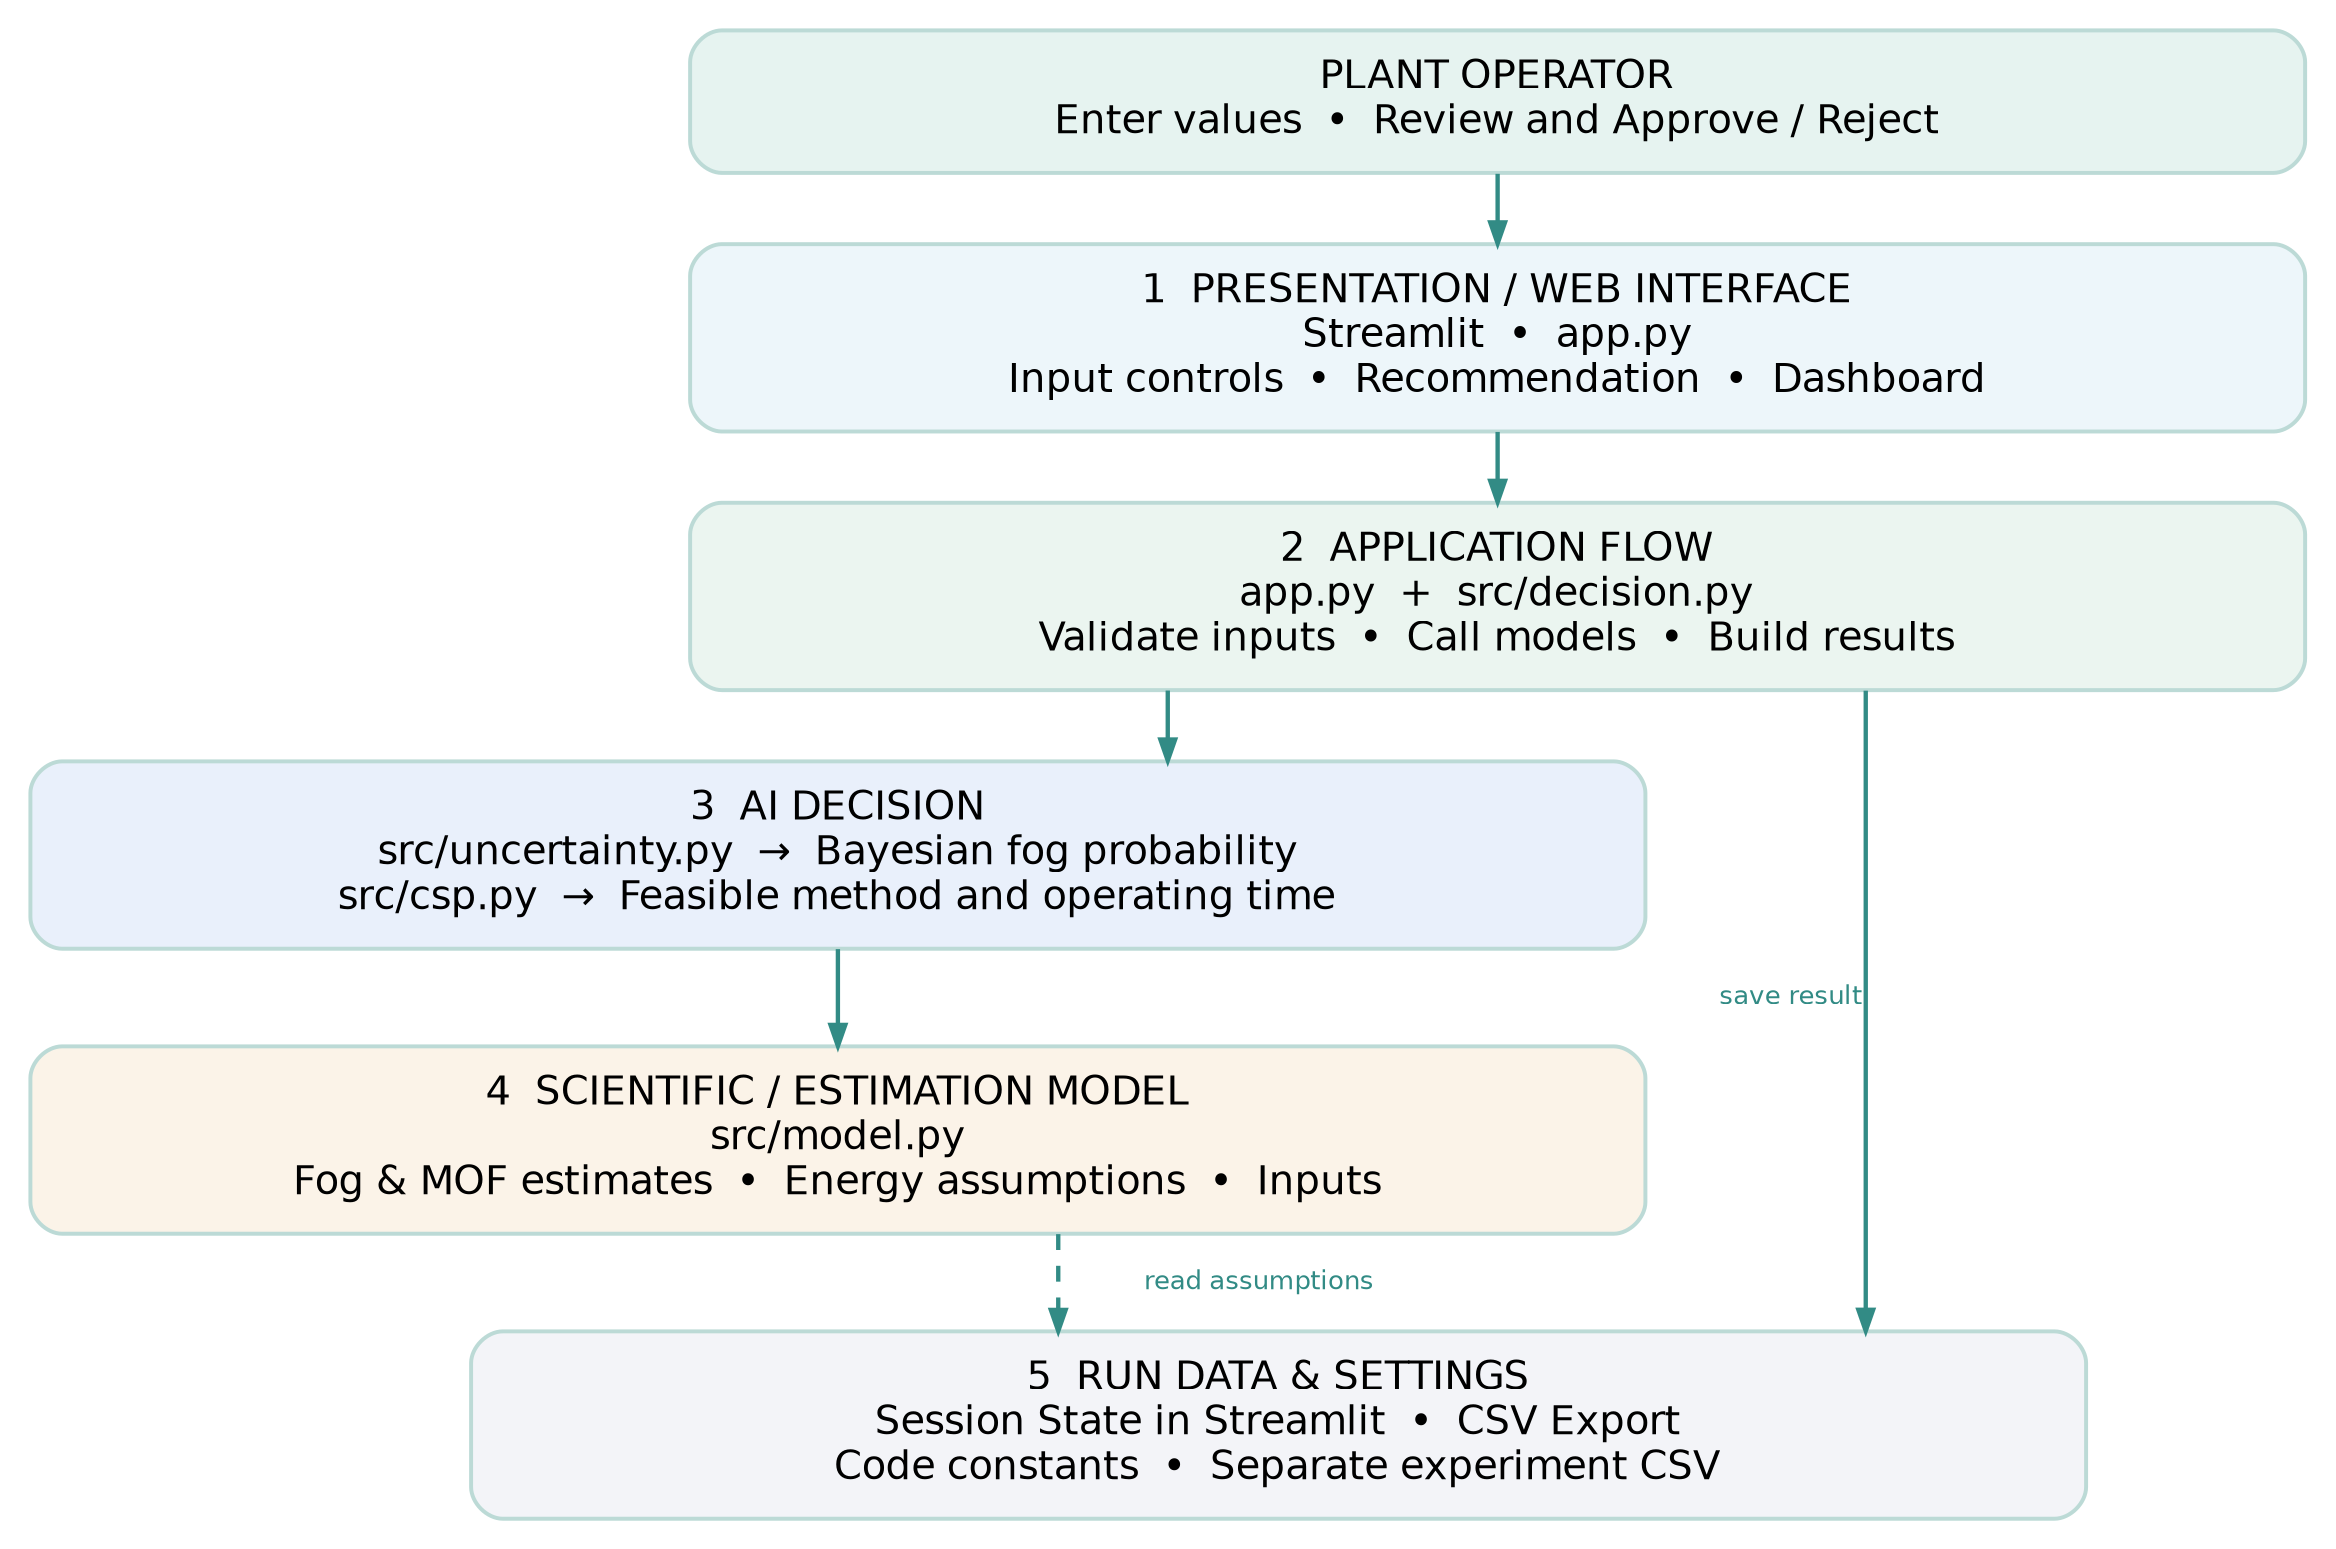
\includegraphics[width=\columnwidth]{figures/architecture.png}
\caption{AquaGent software architecture: user input, Streamlit interface, Bayesian uncertainty, CSP feasibility, simplified reference calculations, and session/export data.}
\label{fig:architecture}
\end{figure}

\clearpage
\section{Methodology}
\subsection{Uncertainty through a Bayesian sensor model}
The model starts with an assumed chance of fog. It updates this value using a fog sensor and assumed sensitivity and specificity. For a positive observation $E^+$,
\begin{equation}
\begin{aligned}
P(F\mid E^+) &= \frac{P(E^+\mid F)P(F)}{D}, \\
D &= P(E^+\mid F)P(F) \\
&\quad + P(E^+\mid \neg F)P(\neg F)
\end{aligned}
\end{equation}
Here, $F$ means fog, $E^+$ means a positive sensor reading, and $P$ denotes probability. The denominator $D$ is written on a second line for readability. A negative sensor reading lowers the estimated chance of fog. If the fog reading is missing, the program keeps the prior estimate and shows a note. These sensor parameters were chosen for demonstration. They were not learned from measurements in Jeddah. This allows us to test how a decision is made when the information is incomplete.

\newpage
\subsection{CSP-based plan filtering and ranking}
Each candidate plan combines a collector type (fog or MOF) with a duration of 1, 2, 4, or 8 hours. The program checks safety, permitted operating time, the electricity budget, and weather-related limits for each method. A plan is rejected if it breaks any hard limit. If all plans are rejected, the system says that no suitable plan is available. Feasible plans are ranked with an illustrative score:
\begin{equation}
S = \frac{L_{\mathrm{demo}}}{1 + E_{\mathrm{demo}}/E_{\mathrm{budget}}},\quad E_{\mathrm{budget}}>0.
\end{equation}
Here, $L_{\mathrm{demo}}$ is estimated water in liters, $E_{\mathrm{demo}}$ is estimated electricity in kWh, and $E_{\mathrm{budget}}$ is the available electricity in kWh. The score is a way to compare simulated options, not a validated measure of cost or real-world performance. The operator still makes the final decision.

\clearpage
\subsection{Reference water and energy calculations}
For fog collection, the model uses assumed liquid-water content (LWC), wind speed $v$, mesh area $A$, and capture efficiency $\eta$:
\begin{equation}
L_{\mathrm{fog}}/h = 3.6\times\mathrm{LWC}\times v\times A\times\eta.
\end{equation}
Here, LWC is in g/m$^3$, $v$ is wind speed in m/s, $A$ is mesh area in m$^2$, and $\eta$ is capture efficiency. The simulated rate is then adjusted using the estimated chance of fog. The MOF reference model scales a daily field observation reported in \citet{song2023}:
\begin{equation}
L_{\mathrm{MOF}}=0.210\,m_{\mathrm{MOF}}\frac{h}{24}.
\end{equation}
Here, $m_{\mathrm{MOF}}$ is the sorbent mass in kg and $h$ is operating time in hours. The value 0.210 L/kg/day comes from a particular published experiment. It does \emph{not} represent a validated hourly rate for Jeddah. For comparison, the code assumes electricity use of 0.10~kWh/h for fog collection and 1.20~kWh/h for MOF. These are demonstration settings. The model does not calculate the full heat required for MOF regeneration or condensation.

\newpage
\section{Experimental Results and Discussion}
\subsection{Software tests and synthetic scenarios}
The code in the confirmed \texttt{AquaGent\_3} package completed 45 automated tests. These tests check the code, not the accuracy of real water production. We reran the ten synthetic scenarios from the same code version and obtained six recommendations, two \texttt{NO\_FEASIBLE\_\allowbreak METHOD} outcomes (no energy and unsafe operation), and two \texttt{SENSOR\_\allowbreak WARNING} outcomes (invalid or missing required humidity). Rejecting an unsafe plan is a correct result, not a failure.

\begin{table}[H]
\centering
\footnotesize
\setlength{\tabcolsep}{3pt}
\begin{tabular}{lrr}
\toprule
Scenario outcome & Count & Meaning\\
\midrule
Recommendation & 6 & Feasible plan\\
No feasible method & 2 & Hard constraint\\
Sensor warning & 2 & Invalid input\\
\midrule
Total & 10 & Synthetic tests\\
\bottomrule
\end{tabular}
\caption{Results from ten predefined simulation scenarios.}
\label{tab:scenarios}
\end{table}
\begin{table}[H]
\centering
\footnotesize
\begin{tabular}{lll}
\toprule
Scenario & Outcome & Method \\
\midrule
Fog detected & Plan & Fog \\
Fog absent & Plan & MOF \\
Fog sensor missing & Plan & MOF \\
Low humidity & Plan & MOF \\
No energy & No plan & None \\
Unsafe & No plan & None \\
Missing humidity & Warning & None \\
Invalid humidity & Warning & None \\
Low sensitivity & Plan & MOF \\
Tight energy & Plan & Fog \\
\bottomrule
\end{tabular}
\caption{Individual decisions in the ten synthetic scenarios. ``No plan'' and ``Warning'' are intended safe outcomes.}
\label{tab:allscenarios}
\end{table}
\clearpage
\paragraph{Reproducible protocol.}
The confirmed \texttt{AquaGent\_3} source was evaluated with \texttt{python -m unittest discover -s tests -v}. Ten synthetic scenarios were rerun from the same code version with \texttt{experiments/run\_simulation.py}. This evaluation counts the outputs and passing tests; it does not measure prediction accuracy against real devices or calibrate Bayesian probabilities. Missing and misleading sensor evidence provides an incomplete-information challenge.



In the predefined fog-detected scenario (85\% humidity, 22\,$^\circ$C, and the script's other default inputs), $P(F)\approx0.829$ and the program selected a four-hour fog plan with 2.865~L and 0.40~kWh. The fog-absent scenario selected MOF for four hours with 0.035~L and 4.80~kWh. Both scenarios use the experiment script's declared inputs. These quantities are illustrative and should not be interpreted as measured hardware performance.



\subsection{Sensitivity to inputs}
\begin{figure}[H]
\centering
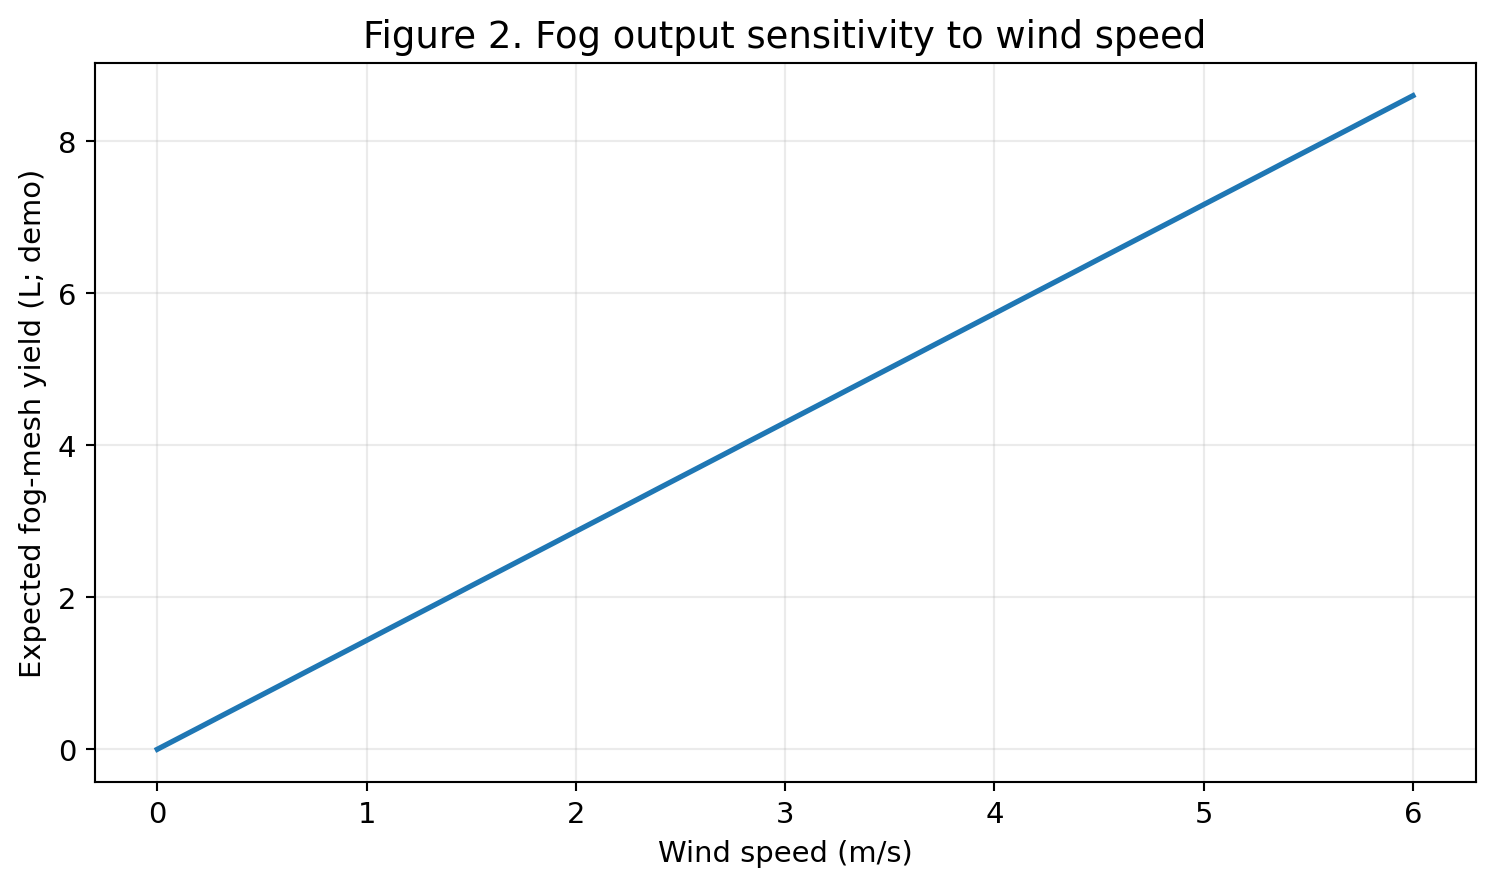
\includegraphics[width=\columnwidth]{figures/fig2_fog_wind.png}
\caption{Fog scenario water output as assumed wind speed changes. The trend follows the simplified model, not a field measurement.}
\label{fig:wind}
\end{figure}

\begin{figure}[H]
\centering
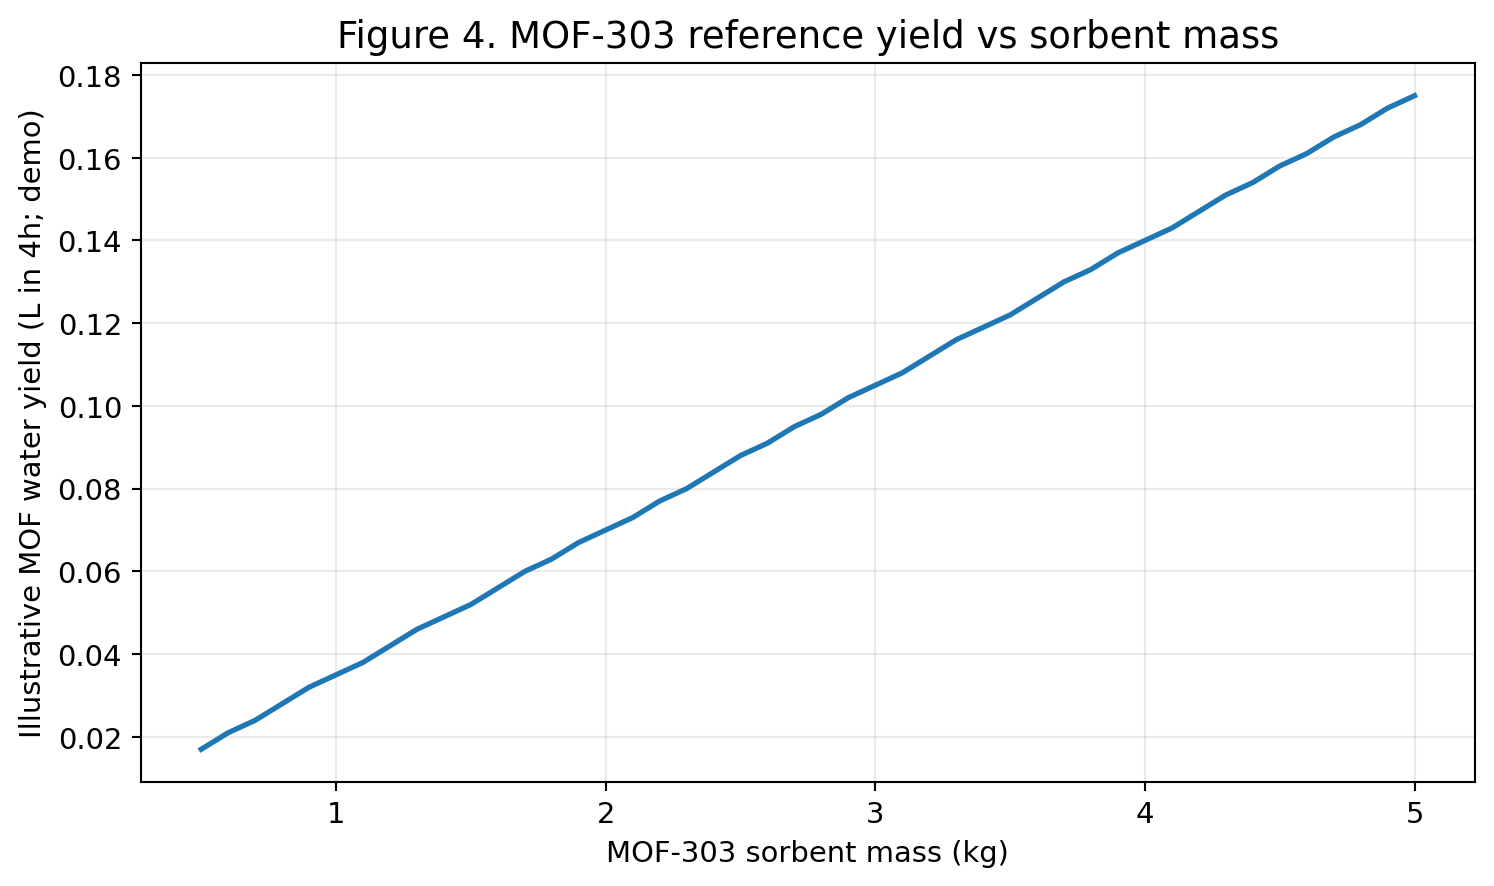
\includegraphics[width=\columnwidth]{figures/fig4_mof_mass.png}
\caption{MOF reference water output versus assumed sorbent mass; the model scales mass linearly.}
\label{fig:mof}
\end{figure}

Under fixed mesh area, capture efficiency, and LWC, the fog equation increases modeled output linearly with wind speed (Fig.~\ref{fig:wind}). The MOF model increases output with sorbent mass (Fig.~\ref{fig:mof}) but does not adjust positive-humidity yield using material adsorption isotherms. This is an important limitation rather than evidence that relative humidity has no physical effect. Differences in assumed device size and energy boundary also make direct numerical performance rankings fragile.

\paragraph{Interpretation.}
Passing these tests means that the program returned the expected output for the tested inputs. It does not prove accuracy under measured field conditions. Comparisons are sensitive to illustrative mesh area, MOF mass, and energy boundaries. For that reason, the current rankings cannot tell us which collector would perform best in Jeddah.

\section{Limitations and Future Work}
Our prototype relies on manual inputs, assumed Bayesian values, simplified water calculations, and example electricity rates. We did not use a measured Jeddah fog dataset, collect real water, run MOF regeneration cycles, or test water quality. The water cannot be called safe to drink without separate quality tests. Before real use, the model would need local weather data, calibrated sensors, confirmed equipment settings, measured water and energy results, and a human safety review. A later MOF model should also account for changes in humidity, temperature, adsorption, and regeneration heat.

\section{Conclusion}
AquaGent brings the project steps into one working prototype: the operator enters conditions, the Bayesian model updates the chance of fog, CSP removes plans that break hard limits, and the interface explains the remaining recommendation. All 45 automated tests passed, and ten simulated cases covered normal operation, missing readings, invalid inputs, and safety limits. This supports the tested software behavior, not the real accuracy of water or electricity estimates. We still need local measurements, calibrated sensors, and a more detailed MOF cycle model before the system could support real equipment decisions.

\section*{Author Contributions}
\noindent\textbf{Zainab Alameri:} Worked jointly with Abubaker on AquaGent, including shared project tasks and reviews.\\
\textbf{Abubaker Baobaid:} Worked jointly with Zainab on AquaGent, including shared project tasks and reviews.\\
Both members must confirm these descriptions and sign the required contribution declaration themselves.

\begin{thebibliography}{9}
\bibitem[Alzahrani and Abdelbaki(2025)]{alzahrani2025} Alzahrani, A. S. and Abdelbaki, A. M. (2025). Fog harvesting implementation as a sustainable water source: a feasibility study in Al-Baha, Saudi Arabia. DOI: 10.1007/s43995-025-00250-w.
\bibitem[Almassad et~al.(2022)]{almassad2022} Almassad, H. A. et al. (2022). Environmentally adaptive MOF-based device enables continuous self-optimizing atmospheric water harvesting. \emph{Nature Communications}, 13, 4873. DOI: 10.1038/s41467-022-32642-0.
\bibitem[Song et~al.(2023)]{song2023} Song, W. et al. (2023). MOF water harvester produces water from Death Valley desert air in ambient sunlight. \emph{Nature Water}, 1, 626--634. DOI: 10.1038/s44221-023-00103-7.
\bibitem[Li et~al.(2022a)]{li2022screening} Li, L. et al. (2022). Machine Learning-Assisted Computational Screening of Metal-Organic Frameworks for Atmospheric Water Harvesting. \emph{Nanomaterials}, 12, 159. DOI: 10.3390/nano12010159.
\bibitem[Wang et~al.(2023)]{wang2023global} Wang, J.-Y. et al. (2023). Global water yield strategy for metal-organic-framework-assisted atmospheric water harvesting. \emph{Cell Reports Physical Science}, 4, 101742. DOI: 10.1016/j.xcrp.2023.101742.
\bibitem[Luo et~al.(2023)]{luo2023} Luo, F. et al. (2023). High-efficient and scalable solar-driven MOF-based water collection unit: From module design to concrete implementation. \emph{Chemical Engineering Journal}, 465, 142891. DOI: 10.1016/j.cej.2023.142891.
\bibitem[Li et~al.(2022b)]{li2022limits} Li, A. C. et al. (2022). Thermodynamic limits of atmospheric water harvesting with temperature-dependent adsorption. \emph{Applied Physics Letters}, 121, 164102. DOI: 10.1063/5.0118094.
\bibitem[P\'erez-S\'anchez and Mulligan(2025)]{perez2025} P\'erez-S\'anchez, J. and Mulligan, M. (2025). Catching Clouds: Mapping the Potential of Fog Water Harvesting in La Palma (Canary Islands). DOI: 10.1007/s41748-025-00955-x.
\end{thebibliography}
\end{document}
